\chapter{Überblick über die Arbeit}\label{sec:experimente}
Im zweiten Teil dieser Arbeit werden die in Kapitel \ref{sec:wissenschaft} theoretisch betrachteten Methoden praktisch auf einer GPU ausgeführt und evaluiert. Der Überblick über das experimentelle Setup wird in Kapitel \ref{sec:setup} vorgestellt. In Kapitel \ref{sec:konzept} wird das Konzept des praktischen Teils der Arbeit erläutert.

\section{Experimentelles Setup}\label{sec:setup}
\subsection{Hardware}
Die Hardware umfasst einen Server mit 4 GPUs.
Von diesen 4 GPUs haben 2 GPUs jeweils den gleichen Typ:
\begin{itemize}
 \item Geforce GTX 1080 Ti
 \item Geforce RTX 2080 Ti 
\end{itemize}

Beide GPU-Typen arbeiten mit der CUDA Version 10.1. 

Während der Vorbereitung auf diese Experimente hat sich gezeigt, dass Experimente mit einer Geforce GTX 1080 Ti mit den Experimenten der Geforce RTX 2080 Ti nicht vergleichbar sind. Weiterhin lässt sich durch das Verwenden von gemischt präzisen Zahlen nur auf der Geforce RTX 2080 ein Geschwindigkeitsvorteil beim Training feststellen. Aus diesen zwei Gründen wurden alle Experimente auf der Geforce RTX 2080 Ti ausgeführt.  


\subsection{Wahl des Frameworks}

Es wird mit pytorch gearbeitet, da pytorch gegenüber anderen Frameworks eine grössere Flexibiltät erlaubt. Ausserdem ist eine fast vollständige Implementierung von PruneTrain in Pytorch geschrieben. Diese wird im nächsten Kapitel untersucht und soweit erweitert, dass es dem Stand im PruneTrain Paper entspricht.

Pytorch bietet mit cudnn und cuda im Hintergrund gute Möglichkeiten die Trainingszeiten einzelner Epochen zu messen und sie so mit einander zu vergleichen.


\subsection{verwendete Netzarchitektur}\label{sec:archi}
Die PruneTrain Implementierung hat initial mehrere verschiedene Netzarchitekturen zur Auswahl:
\begin{itemize}
 \item AlexNet
 \item ResNet 32/50
 \item vgg 8/11/13/16
 \item mobilenet
\end{itemize}

Diese Auswahl an Netzarchitekturen ist zu umfangreich, um alle diese Architekturen auf den vorgestellten Methoden zu evaluieren. Daher wird im Rahmen dieser Arbeit nur auf ResNet gearbeitet. Diese Entscheidung liegt daran, dass Resnets durch ihre Kurzschlussverbindungen gut mit sehr tiefen Netzstrukturen unmgehen können, ohne grosses Klassifikationsleistungsverluste dank Overfitting. Dies ist vorallem wichtig, wenn das Netz mit Hilfe des Operator für tieferes Netz noch tiefer gemacht werden soll. Die ResNet Struktur wird in der Implementierung so verändert, dass angeben werden kann wie tief das Netz sein soll. Das ResNet wird hier nicht mehr nur mit einer Zahl identifiziert sondern es wird angegeben, wieviele
\begin{itemize}
 \item $s$: Anzahl an Phasen, die das ResNet hat
 \item $N=[n_1, \ldots, n_S]:$ Anzahl von Blöcken pro Phase 
 \item $l$: Anzahl von (Conv+Batch)-Layer pro Block
 \item $[k_1, \ldots,k_S ]:$ Breite der Schichten je Phase
 \item $b$: Boolean Parameter, der angibt ob die Blöcke im Netz die Bootleneck-Eigenschaft haben
\end{itemize}
das jeweilige ResNet hat. Diese Vorgehensweise hat den Vortei, dass für ein im Verlauf tieferes beziehungweise breitere Netz eine Vergleichsmöglichkeit besteht. Dies bedeutet, dass das Netz welches im Verlauf entsteht auch direkt erstellt werden kann.


\subsection{Baseline Netz}\label{sec:baseline}

Um die Ergebnisse der Experimente in den folgenden Kapiteln einschätzen zu können wird ein ResNet, ohne Anpassungen um Trainingszeit zu sparen, trainiert. In Tabelle \ref{tab:baseline} ist die Struktur dieses Netze zu sehen. Das breite Baseline-Netz wird dabei für die Evaluierung des Beschneiden des Netzes verwendet. Das schmallere Baseline-Netz wird für die Evaluierung der Methoden, die das Netz breiter machen verwendet.

Das Netz hat drei Phasen $(s=3)$, wobei jeder der Phasen 5 Blöcke hat $(N=[5,5,5])$. Pro Basisblock sind zwei (Conv+Batch)-Schichten vorhanden $(l=2)$. Bei einem Übergangsblock, der als erster Block in einer neuen Phase bei einer Vergrösserung der Bereit beim Phasenübergang genutzt wird ist eine (Conv+Batch)-Schicht mehr vorhanden. Eine grafische Darstellung der Blöcke ist in Abbildung \ref{abb:blocks} zu sehen.




\begin{figure}[]
   \begin{minipage}[b]{.4\linewidth} % [b] => Ausrichtung an \caption
      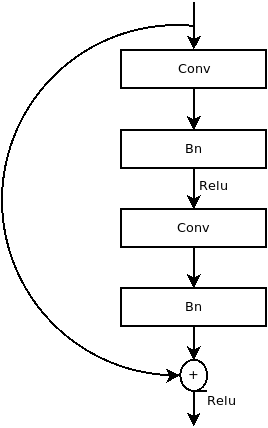
\includegraphics[width=0.8\linewidth]{KapitelPartB/Images/Basisblock.png}
      \caption{Basisblock}
   \end{minipage}
   \hspace{.1\linewidth}% Abstand zwischen Bilder
   \begin{minipage}[b]{.4\linewidth} % [b] => Ausrichtung an \caption
      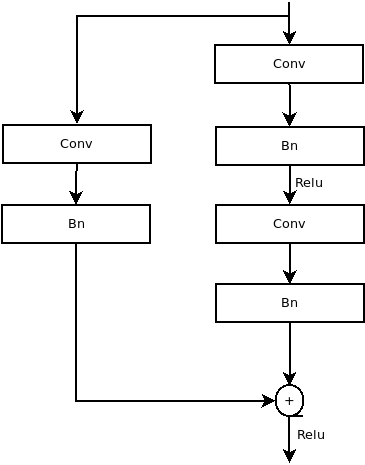
\includegraphics[width=0.8\linewidth]{KapitelPartB/Images/Ubergangsblock.png}
      \caption{Übergangsblock}
   \end{minipage}
   \caption{Grafische Darstellung Basis- und Übergangsblock}
   \label{abb:blocks}
\end{figure}

\begin{table}[]
\begin{tabular}{|l|l|l|l|l|l|}
\hline
      &                & \multicolumn{2}{c|}{breites Baseline-Netz} &\multicolumn{2}{c|}{schmalles Baseline-Netz} \\ 
Phase & Schicht/Block  & \#Eingangs- & \#Ausgangs-       & \#Eingangs- & \#Ausgangs-    \\
      &                & \multicolumn{2}{c|}{kanäle}     & \multicolumn{2}{c|}{kanäle}  \\ \hline
      & Conv 1 + Bn 1  & 3                & 16           & 3           & 8              \\ \hline \hline
1     & Basisblock     & 16               & 16           & 8           & 8              \\ \hline
      & Basisblock     & 16               & 16           & 8           & 8              \\ \hline
      & Basisblock     & 16               & 16           & 8           & 8              \\ \hline
      & Basisblock     & 16               & 16           & 8           & 8              \\ \hline
      & Basisblock     & 16               & 16           & 8           & 8              \\ \hline \hline
2     & Übergangsblock & 16               & 32           & 8           & 16             \\ \hline
      & Basisblock     & 32               & 32           & 16          & 16             \\ \hline
      & Basisblock     & 32               & 32           & 16          & 16             \\ \hline
      & BasisBlock     & 32               & 32           & 16          & 16             \\ \hline
      & BasisBlock     & 32               & 32           & 16          & 16             \\ \hline \hline
3     & Übergangsblock & 32               & 64           & 16          & 32             \\ \hline
      & Basisblock     & 64               & 64           & 32          & 32             \\ \hline
      & Basisblock     & 64               & 64           & 32          & 32             \\ \hline
      & Basisblock     & 64               & 64           & 32          & 32             \\ \hline
      & Basisblock     & 64               & 64           & 32          & 32             \\ \hline \hline
      & Linear         & 64               & 10           & 32          & 10             \\ \hline
\end{tabular}
\caption{Struktur des Netzes}
\label{tab:baseline}
\end{table}


\subsubsection{Evaluierung des breiteren Baseline-Netzes}
Das Training wird über 180 Epochen durchgeführt. Es werden 5 Experimente durchgeführt. Dabei ergibt sich der in Abbildung \ref{abb:baseAcc1} gezeigte Verlauf der Validierungs-Accuracy für Experiment vier. Bei diesem Training wurde über die gesamten 180 Epochen mit einer Lernrate von 0.1 trainiert. Mit einem Ergebnis von durchschnittlich 81.11 \% über fünf Experimente ist diese Ergebnis leider nicht zufriedenstellend. 

Eine Verkleinerung der Lernrate kann dieses Ergebnis verbessern \cite{CNNBook}. In Abbildung \ref{abb:baseAcc2} wird dargestellt, wie sich der Verlauf ändert durch eine Anpassung der Lernrate bei Epoche 93 und 150. In diesen beiden Epochen wird die Lernrate jeweils auf ein Zehntel verkleinert. 

In Abbildung \ref{abb:baseAcc3} ist ein Boxplot dargestellt, der die Accuracy von jeweils fünf Experimenten mit oder ohne Anpassung der Lernrate vergleicht. Es ergibt sich eine deutliche Verbesserung der Accuracy des Baseline-Netzes von 81.24 \% auf 91.89 \% durch diese Anpassung. 
\color{blue1}
Hier wurden die Epochen, zu denen die Lernrate verkleinert wurde manuell ausgesucht. 


Da die Accuracy sich mittels der Verkleinerung der Lernrate verbessert und somit bei direktem Verändern der Struktur im aktuellen Modell ungenutztes Potential verbleibt wird das Verkleinern der Lernrate angewendet, bevor die Struktur verändert wird.


Somit ist es an dieser Stelle notwendig entweder ein geeignetes bestehendes Verfahren zur automatischen Anpassung der Lernrate zu finden, welches auch mit der Situation eines nicht auf einen bestimmten Accuracy Wert konvergierendes Netz klarkommt. 

Bestehende Verfahren zur Anpassung der Lernrate:
\begin{itemize}
 \item Adam
 \item AdaGrad
\end{itemize}




\color{black}

\begin{comment}
Aufgrund dieser Verbesserung werden die Experimente mit Anpassung der Lernrate als Grundlage zum Vergleich mit den Experimenten in den weiteren Kapiteln herangezogen. Sie werden in diesen Kapitel nur mit Baseline-Netz bezeichnet.
\end{comment}
\begin{figure}
     \centering
     \subfloat[][]{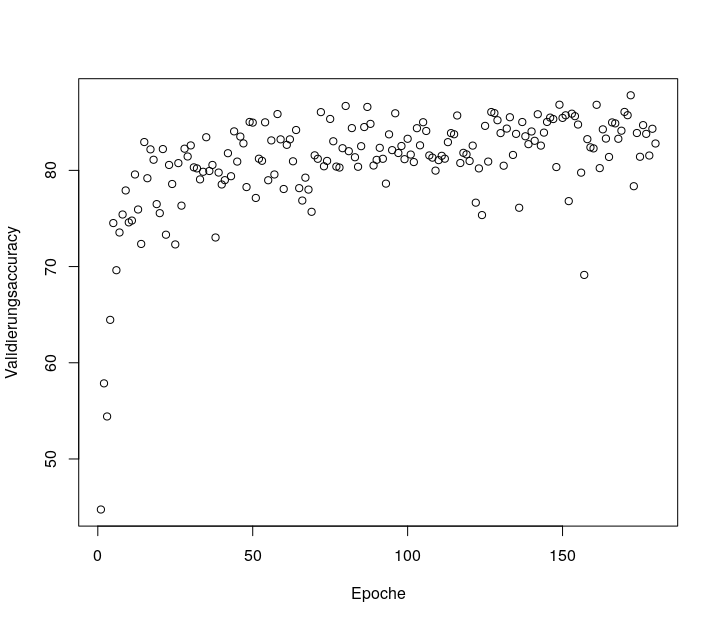
\includegraphics[width=.49\textwidth]{KapitelPartB/Images/BaseAcc1.png}\label{abb:baseAcc1}}
     \subfloat[][]{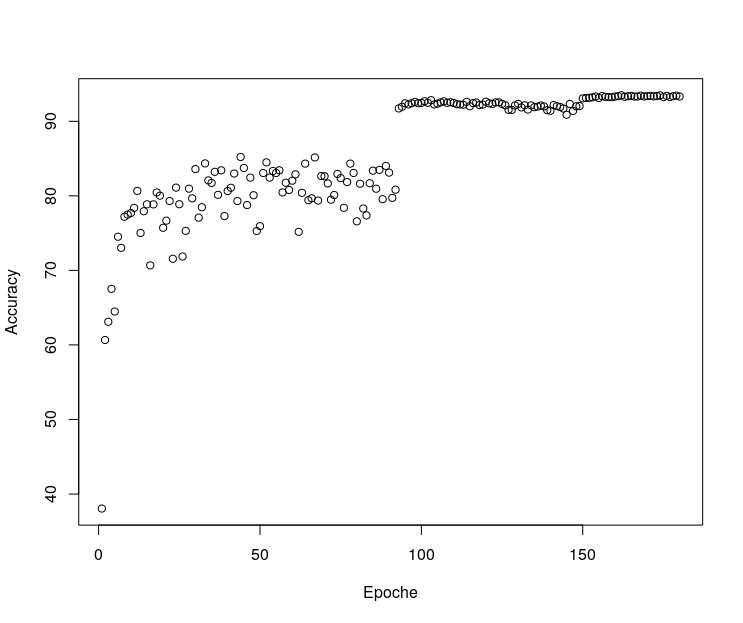
\includegraphics[width=.49\textwidth]{KapitelPartB/Images/BaseAcc.png}\label{abb:baseAcc2}}\\
     \subfloat[][]{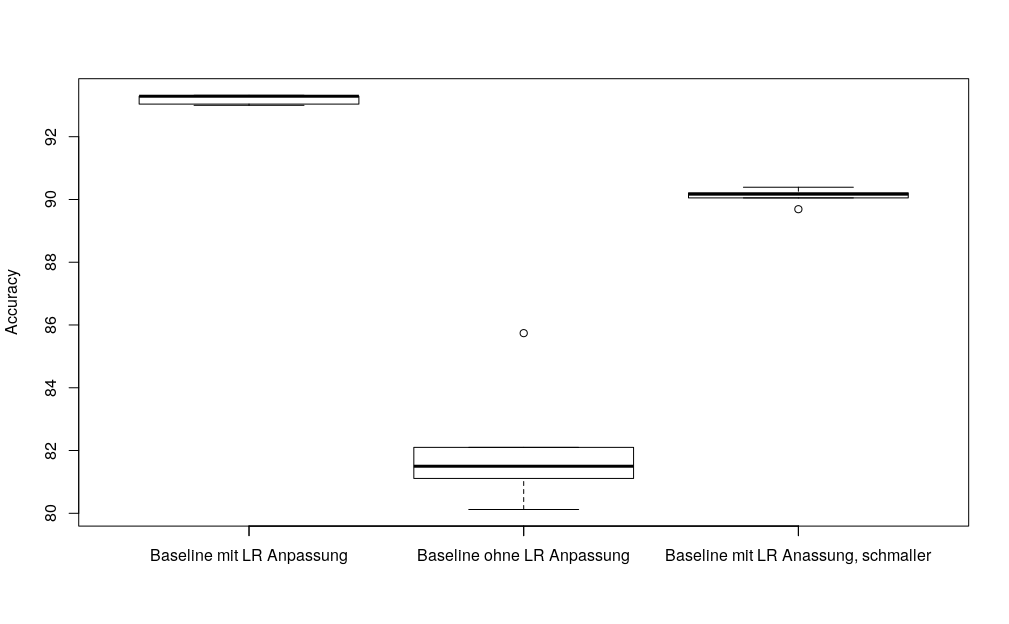
\includegraphics[width=.49\textwidth]{KapitelPartB/Images/BaseAcc3.png}\label{abb:baseAcc3}}
     \caption{Vergleich zwischen (a) Baseline-Netz ohne Anpassung der Lernrate und (b) Baseline-Netz mit Anpassung der Lernrate in Epoche 93 und 150. (c)  Boxplot der Accuracys}
     \label{abb:BaseAcc}
\end{figure}

Ein weiteres Vergleichskriterium neben der Accuracy sind die durchschnittlichen Trainingszeiten pro Epoche. Für jedes Experiment wird die durchschnittliche Dauer einer Trainingsepoche mittel des arithmetiscen Mittels berechnet.
Die Durchschnittswerte über alle 180 Epoche sind für die zehn Baseline Experimente sind in Tabelle \ref{tab:baselineTime} aufgelistet. Die Durchschnittswerte liegen sehr nah beeinander, der Unterschied zwischen dem grössten und dem kleinsten Durchschnittswert liegt bei 0,28. Damit ergeben sich zwischen den zehn Experimenten keine signifikante Unterschiede. Es wird daher mit Experiment vier eines der Experimente mit Anpassung der Lernrate ausgesucht um für die folgenden Experimente/ Kapitel als Vergleich zu dienen.
\begin{table}[h]
\begin{tabular}{|l|l|l|l|l|l|l|l|l|l|l|} \hline
           & \multicolumn{5}{c|}{Experimente ohne Anpassung}&\multicolumn{5}{c|}{Experimente mit Anpassung} \\
           &\multicolumn{5}{c|}{der Lernrate} &\multicolumn{5}{c|}{der Lernrate}\\
           & 1       & 2      & 3      & 4       & 5       & 1      & 2     & 3      & 4     & 5  \\ \hline 
$\mu$      & 19,49   & 19,53  & 19,50  & 19,48   & 19,84   & 19,57  & 19,56 & 19,53  & 19.53 & 19.62 \\ \hline
\end{tabular}
\caption{Tabelle für Durchschnittswerte und Standardabweichungen der Trainingszeiten der Experimente}
\label{tab:baselineTime}
\end{table}
\color{black}
\subsubsection{Evaluierung des schmalleren Baseline-Netzes}

\todo[inline]{schmalles Netz ohne LR-Anpassung}
Das schmallere Baseline-Netz wird verwendet, um für MorphNet und Net2Net eine schmalle Variante zu haben. Der Grund hierfür ist, dass bei einer durchschnittlichen Accuracy von 93,19 \% des breiten Baseline-Netzes nicht mehr viel Raum für Verbesserungen bleibt. In Abbildung \ref{abb:baseAcc3} sind die Experimente für das breite und schmalle Baseline-Netz mit der Anpassung der Lernrate gegenüber gestellt. Der Unterschied vom breiten zum schmallen Netz ist ein Accuracy-Verlust von 3,1 \%.    


In Abbildung \ref{abb:baseAccS1} ist abgebildet, wie sich die Accuracy für das schmallere Netz verhält, bei der gleichen Anpassung der Lernrate wie beim breiteren Baseline-Netzen. Der Unterschied in der Accuracy zwischen dem schmallen und breiten Baseline-Netz ist in Abbildung \ref{abb:baseAccS2} abgebildet.


\begin{figure}
     \centering
     \subfloat[][]{ 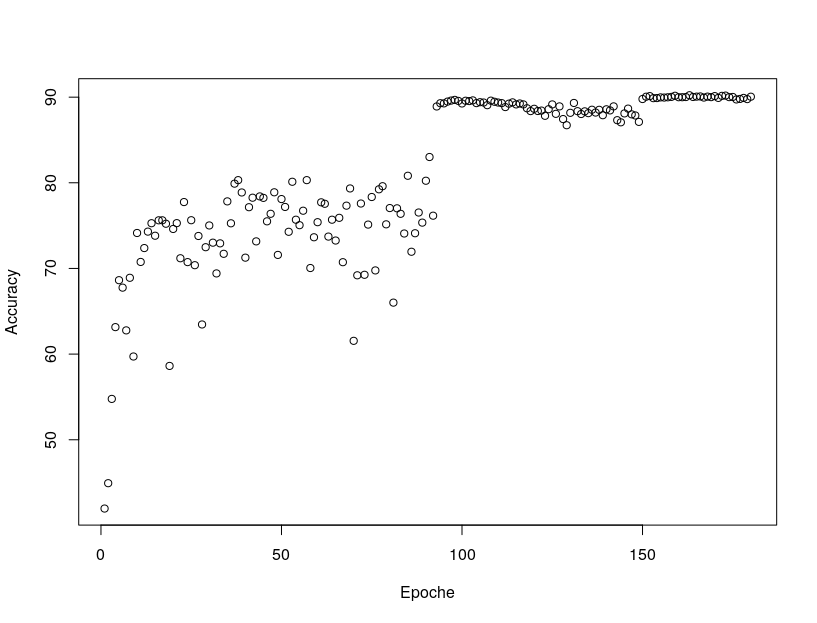
\includegraphics[width=0.5\textwidth]{KapitelPartB/Images/baseAccS.png}\label{abb:baseAccS1}}
     \subfloat[][]{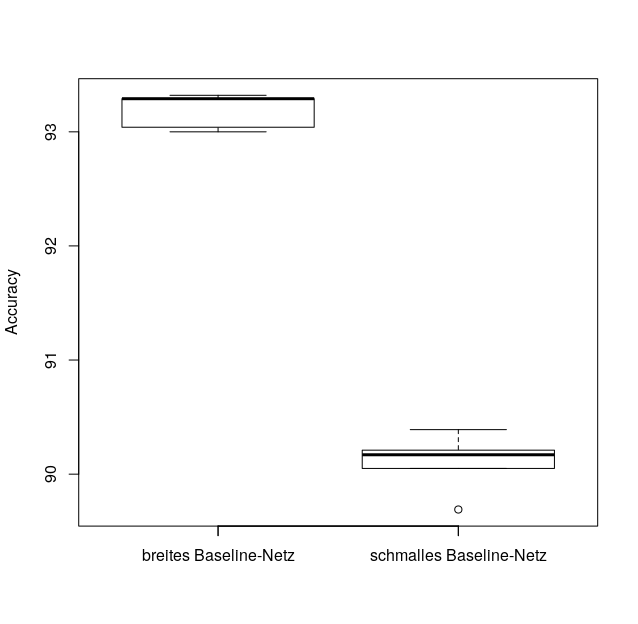
\includegraphics[width=.49\textwidth]{KapitelPartB/Images/baseAccSHisto.png}\label{abb:baseAccS2}}
     \caption{}
     \label{abb:BaseAccS}
\end{figure}


\color{black}

\section{Konzept}\label{sec:konzept}
\todo[inline]{Überarbeiten}
In den nachfolgenden Kapiteln wird MorphNet mit einer Kombination aus PruneTrain und Net2Net verglichen. MorphNet ist eine Technik, bei der die Struktur des Netzes durch Wiederholtes Verbreitern des Netzes und Verkleinern des Netzes mittels eines Regularisierers gelernt wird.
PruneTrain beschneidet das Netz so, dass unwichtige Gewichte auf Null gesetzt werden mit dem Ziel ganze Kanäle auf Null zu setzen um diese zu Entfernen. Mit der Entfernung von Kanälen und falls alle Kanäle einer Schicht auf Null gesetzt wurde auch ganzen Schichten, soll Trainingszeit gespart werden bei möglichst geringem Accuracy Verlust.



Um diese beiden Methoden vergleichen zu können werden hier zunächst grundlegende Rahmenbedingungen festgelegt.
Beide Methoden bekommen drei verschieden ausgeprägte Netzwerke mit jeweils drei Phasen:
\begin{itemize}
 \item Netz mit $N=[3,3,3]$ und $K=[8,16,32] $
 \item Netz mit $N=[4,4,4]$ und $K=[4,8,16] $
 \item Netz mit $N=[4,4,4]$ und $K=[8,16,32] $
\end{itemize}
Dabei können mehrere Durchgänge der Netzvergrösserung durchlaufen werden. Beschränkt sind diese Durchläufe nicht direkt in der Anzahl, da hier beide Methoden verschieden lange Phasen zwischen den Netzvergrösserungsschritten haben. Um trotzdem zeitlich ein Begrenzung zu haben ist es beiden Methonden nicht erlaubt nach 4 Stunden Laufzeit das Netz nochmal zu vergrössern.

Um für die Netze eine Beschränkung zu haben sind maximal die Anzahl Parameter/Flops erlaubt, die das breite Baseline Netz hat.

MorphNet wird in Kapitel \ref{sec:morphexperimente} evaluiert. In Kapitel \ref{sec:ptexperimente} wird PruneTrain so evaluiert, wie es in der vorgefertigten Implementierung \footnote{\url{https://bitbucket.org/lph\_tools/prunetrain/src/master/}} geschrieben wurde. In Kapitel \ref{sec:ptnew} wird die Erhöhung der Batchgröße bei Beschneiden des Netzes evaluiert.

In Kapitel \ref{sec:net2netexperimente} wird Net2Net evaluiert.
In Kapitel \ref{sec:ptpnet2net} wird die Vorgehensweise zum Kombinieren von PruneTrain und Net2Net beschrieben sowie die Kombination evaluiert.

Der Vergleich der beiden Methoden wird in Kapitel \ref{sec:vergleich} vollzogen.
\todo[inline]{nur wenn noch Zeit übrig: In Kapitel 8 werden die Ergebnisse aus 6.3 auf einem anderen Datensatz verifiziert. auch wenn noch Zeit: Prüfe wie sich die additiven Verfahren auf 6.3 auswirken Zuletzt werden noch additive Verfahren vorgetellt, welche die Trainingszeit zusätzlich minimieren können. Eine dieser Verfahren, welches in Kapitel evaluiert wird, spart Zeit durch die Verwendung von gemischt präzisen Zahlenformaten.
Ein weiteres additives Verfahren in Kapitel  überprüft in wiefern mit Hilfe einer adaptiven Anpassung der Lernrate die Batchgröße sinvoll so angepasst werden kann, dass die ganze GPU genutzt werden kann.}






